\documentclass[11pt,t]{beamer}
\usetheme{metropolis}
\metroset{progressbar=frametitle,numbering=fraction}
\setbeamertemplate{frame numbering}{\insertframenumber/\insertmainframenumber} % the total leaves out the backup after \appendix
\usefonttheme[onlymath]{serif} % serif math: proper primes, hats and italics
\usepackage{bm}
\usepackage{amsmath,amssymb,amsfonts}
\usepackage{mathrsfs}
\usepackage{booktabs}
\usepackage{multirow}
\usepackage{graphicx}
\usepackage{xcolor}
\usepackage{tikz}
\usetikzlibrary{calc,positioning,decorations.pathmorphing,arrows.meta}
\setbeamercolor{block title}{use=normal text, fg=normal text.fg,bg=normal text.bg!80!fg}
\graphicspath{{./figures/}{./logo/}}

%%%%%%%%%%%%% Macros %%%%%%%%%%%%%
\newcommand{\rmi}{\mathrm{i}}
\newcommand{\rmd}{\mathrm{d}}
\newcommand{\DM}{\mathrm{DM}}

\title{Generative Modeling of\\ Critical Dynamics}
\subtitle{}

\date{October 16, 2026}
\author{Yang-yang Tan}
\titlegraphic{%
  \begin{tikzpicture}[remember picture, overlay]
    % Top-left: workshop name
    \node[anchor=north west, inner sep=0pt, font=\normalsize\bfseries, text=burgundy]
      at ([xshift=0.6cm,yshift=-0.5cm]current page.north west)
      {Particle Theory Group, CCS, University of Tsukuba};
    % Bottom-right: UTokyo + IPI (aligned with author/date)
    \node[anchor=south east, inner sep=0pt] (utokyo) at ([xshift=-0.6cm,yshift=4.5cm]current page.south east) {%
      \raisebox{-0.5\height}{\includegraphics[height=3em]{UTokyo_Logotype_A_Color_RGB20240401.png}}%
      \hspace{0.4em}\rule[-0.9em]{0.4pt}{2em}\hspace{0.4em}%
      \raisebox{-0.5\height}{\includegraphics[height=2.3em]{ipilogo.png}}%
    };
    % Below UTokyo/IPI: RIKEN + iTHEMS (no separator)
    \node[anchor=north east, inner sep=0pt] at ([yshift=-0.5em]utokyo.south east) {%
      \raisebox{-0.5\height}{\includegraphics[height=2em]{logo_riken.pdf}}%
      \hspace{0.6em}%
      \raisebox{-0.5\height}{\includegraphics[height=2em]{logo_dark.pdf}}%
    };
    % Bottom-right corner: DM-QFT collaboration logo and website
    \node[anchor=south east, inner sep=0pt, align=right] at ([xshift=-0.6cm,yshift=0.7cm]current page.south east) {%
      \raisebox{-0.5\height}{\includegraphics[height=2.4em]{dm_qft_logo.png}}\hspace{0.35em}{\Large\bfseries\color{dmqft}DM-QFT}\\[0.25em]
      {\small\color{dmqft}dm-qft.github.io/homepage}};
  \end{tikzpicture}%
}

\definecolor{burgundy}{RGB}{127, 0, 32}
\definecolor{Kleinblue}{RGB}{0, 47, 167}
\definecolor{dmqft}{RGB}{36, 108, 131} % median ink colour of logo/dm_qft_logo.png
\newcommand{\running}[1]{\textcolor{burgundy}{#1}}
\newcommand{\kb}[1]{{\bfseries\color{Kleinblue} #1}}
% references pinned to the bottom of the page, independent of the frame content
\makeatletter
\newcommand{\refs}[1]{%
  \begin{tikzpicture}[remember picture, overlay]
    \node[anchor=south west, inner sep=0pt, align=flush left,
          text width=\dimexpr\textwidth-1.4cm\relax]
      at ([xshift=\beamer@leftmargin, yshift=0.6cm]current page.south west)
      {\raggedright\tiny\color{black!65} #1\par};
  \end{tikzpicture}}
\makeatother
\newcommand{\rtag}[1]{\textcolor{burgundy}{\textbf{#1}}}

\tikzset{
  stage/.style={
    rectangle, rounded corners=3pt,
    draw=#1!80, fill=#1!12, line width=0.8pt,
    minimum width=2.8cm, minimum height=1.7cm,
    align=center, font=\small\bfseries, text=#1!50!black,
    inner sep=4pt
  },
  tlarrow/.style={
    ->, >=stealth, line width=1.4pt, draw=gray!55,
    shorten >=2pt, shorten <=2pt
  }
}

\begin{document}
\begin{frame}[plain,noframenumbering,t]
  \inserttitlegraphic\par
  \vspace*{0.5cm}
  {\LARGE\bfseries \inserttitle\par}
  \vspace{0.4em}
  {\color{orange}\rule{\textwidth}{0.4pt}\par}
  \vspace{1.4em}
  {\normalsize\bfseries \insertauthor\par}
  \vspace{0.6em}
  {\small IPI, The University of Tokyo\par}
  \vspace{0.4em}
  {\small with \textbf{Lingxiao Wang},\\
  and \textbf{Gert Aarts}, \textbf{Diaa E.\ Habibi}, \textbf{Biagio Lucini} [arXiv:2607.08505],\\
  and \textbf{Jinyang Li} [arXiv:2610.00546]\par}
  \vspace{0.3em}
  {\normalsize \insertdate\par}
\end{frame}

\begin{frame}{Outline}
  \tableofcontents
\end{frame}

% ================================================================ Intro
\section{Critical phenomena and universality}
% ---------------------------------------------------------------- 1
\begin{frame}{Critical phenomena across physics}
  \begin{columns}[T,onlytextwidth]
    \begin{column}{0.36\textwidth}
      \centering
      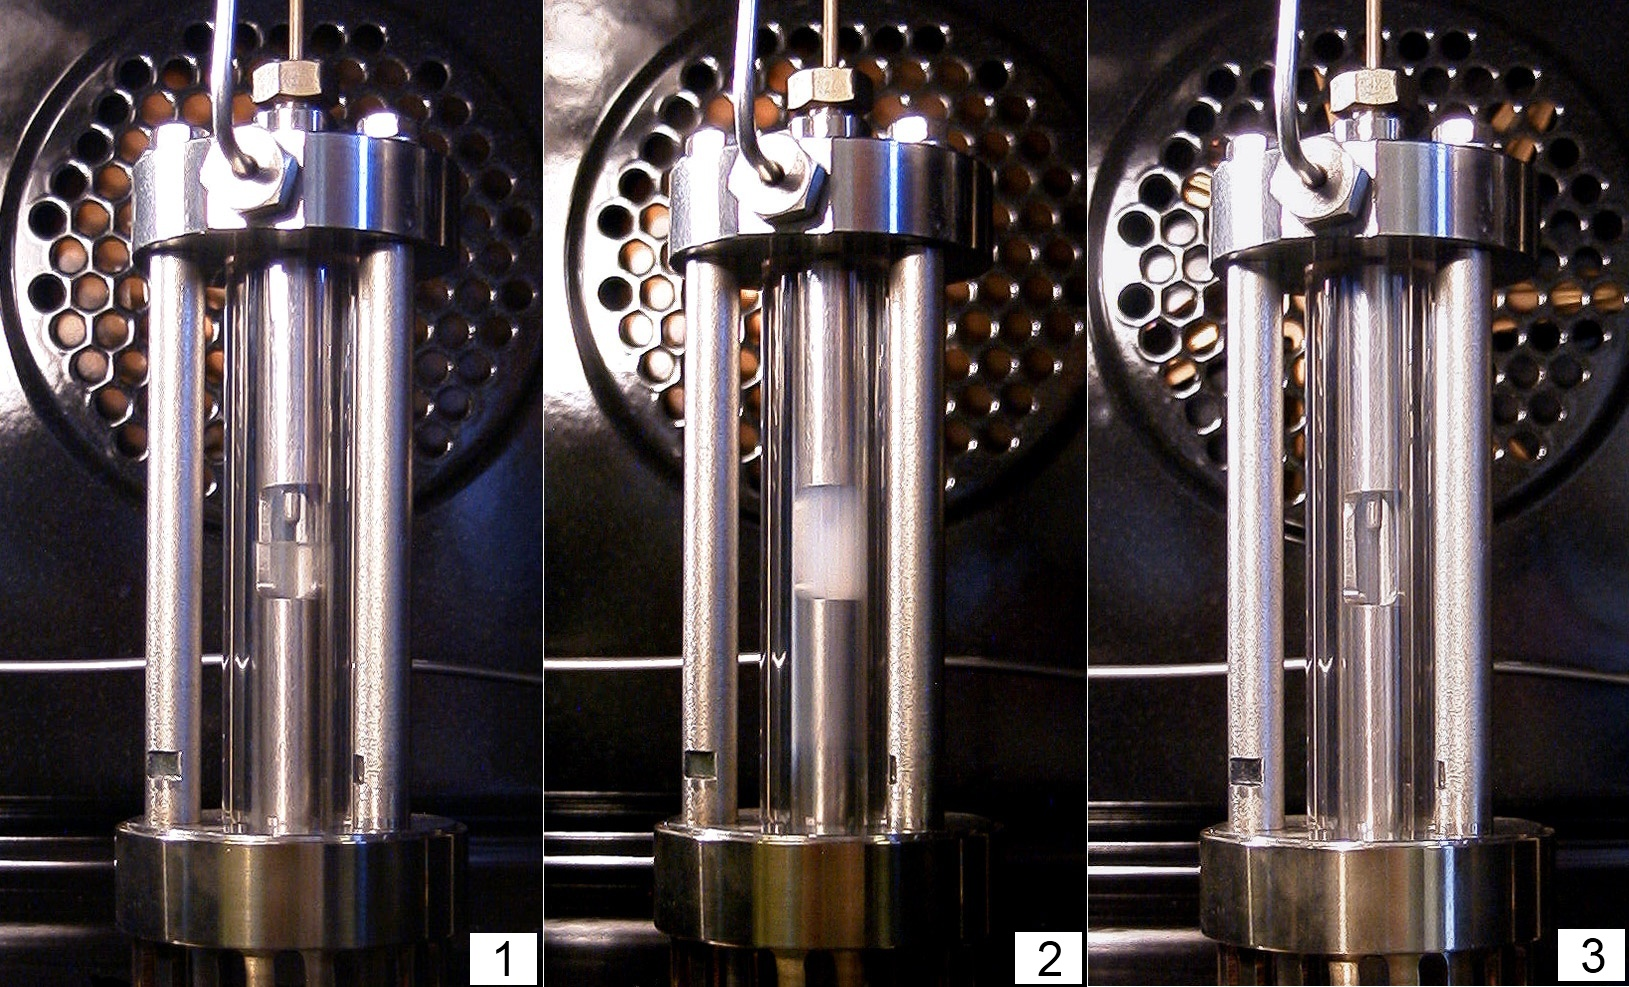
\includegraphics[height=2.15cm]{critical_opalescence_ethane.jpg}\\[0.1em]
      {\scriptsize liquid--gas: ethane at $T_c$}
    \end{column}
    \begin{column}{0.31\textwidth}
      \centering
      \includegraphics[height=2.15cm]{gpmv_membrane_critical.png}\\[0.1em]
      {\scriptsize cell membranes, $d=2$}
    \end{column}
    \begin{column}{0.31\textwidth}
      \centering
      \includegraphics[height=2.15cm]{qcd_phase_diagram_bhalerao.png}\\[0.1em]
      {\scriptsize QCD: critical end point}
    \end{column}
  \end{columns}
  \vspace{1.0em}
  \begin{columns}[T,onlytextwidth]
    \begin{column}{0.56\textwidth}
      \centering
      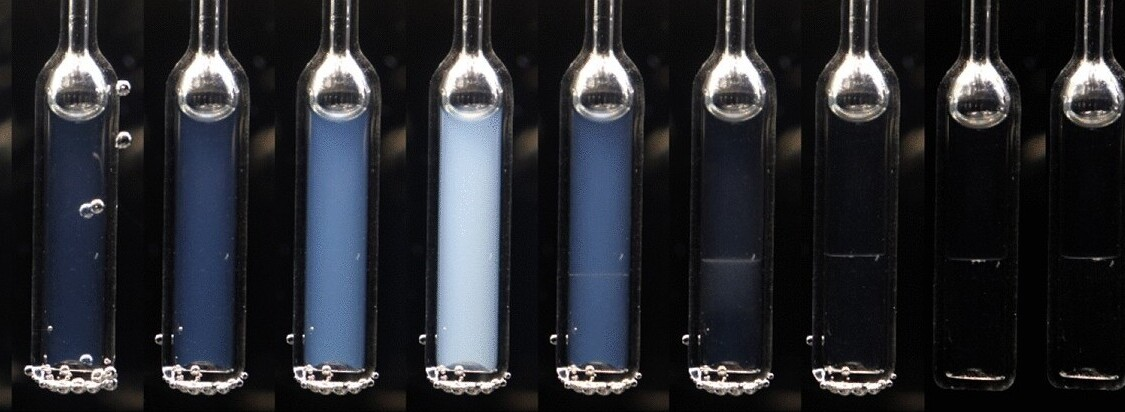
\includegraphics[height=2.0cm]{picoline_d2o_opalescence.jpg}\\[0.1em]
      {\scriptsize binary mixture 3-picoline--D$_2$O at $T_c$}
    \end{column}
    \begin{column}{0.42\textwidth}
      \footnotesize\raggedright
      \kb{Universal features}\\[0.2em]
      no characteristic length, $\xi\to\infty$\\
      fluctuations on every scale\\
      power-law singularities at $T_c$\\
      $\chi\sim|T-T_c|^{-\gamma}$, $\xi\sim|T-T_c|^{-\nu}$
    \end{column}
  \end{columns}
  \refs{%
    \rtag{Ethane:} Horstmann, Wikimedia Commons.\quad
    \rtag{Membranes:} Gray, Karslake, Machta, Veatch, Biophys.\ J.\ 105, 2751 (2013).\quad
    \rtag{Mixture:} Kalabi\'nski, Drozd-Rzoska, Rzoska, EPJ E 45, 73 (2022).\quad
    \rtag{QCD:} Bhalerao, doi:10.5170/CERN-2014-001.219; Stephanov, Rajagopal, Shuryak, PRL 81, 4816 (1998).}
\end{frame}

% ---------------------------------------------------------------- 2
\begin{frame}{Universality}
  \begin{columns}[T,onlytextwidth]
    \begin{column}{0.46\textwidth}
      \centering
      \includegraphics[width=\linewidth]{coexistence_universality.pdf}\\[-0.1em]
      {\scriptsize eight fluids, one coexistence curve}\\[0.2em]
      {\normalsize \alert{experimental data}}
    \end{column}
    \begin{column}{0.52\textwidth}
      \centering
      {\scriptsize
      \renewcommand{\arraystretch}{1.05}
      \setlength{\tabcolsep}{3pt}
      \begin{tabular}{lccc}
        \toprule
        & $\beta$ & $\gamma$ & $\nu$ \\
        \midrule
        fluids & $0.32$--$0.33$ & $1.23$--$1.25$ & $0.62$--$0.63$ \\
        mixtures & $0.32$--$0.33$ & $1.23$--$1.25$ & $0.62$--$0.64$ \\
        magnets & $0.32$--$0.33$ & $1.24$--$1.25$ & $0.62$--$0.64$ \\
        \alert{3D Ising} & $0.3265$ & $1.2372$ & $0.6301$ \\
        \bottomrule
      \end{tabular}}

      \vspace{0.9em}
      \footnotesize\raggedright
      \kb{Only $d$ and symmetry matter}\\[0.2em]
      fluids, mixtures, uniaxial magnets\\
      and the QCD critical end point:\\
      \alert{all 3D Ising}\\
      cell membranes: 2D Ising, same story

      \vspace{0.5em}
      \kb{Lattice $\phi^4$ is the minimal representative of the class}
    \end{column}
  \end{columns}
  \refs{%
    \rtag{Coexistence curves:} Guggenheim, J.\ Chem.\ Phys.\ 13, 253 (1945); data from the NIST Chemistry WebBook, line $\rho_\pm/\rho_c=1+\tfrac34(1-T/T_c)\pm\tfrac74(1-T/T_c)^{1/3}$.\quad
    \rtag{Exponents:} Pelissetto, Vicari, Phys.\ Rept.\ 368, 549 (2002).}
\end{frame}

% ---------------------------------------------------------------- 3
\begin{frame}{Dynamic universality}
  \centering
  % 四列在 8pt 下宽 337pt，超出 307pt 文字宽；7pt 刚好放下（300pt）
  {\fontsize{7}{8.5}\selectfont
  \renewcommand{\arraystretch}{1.05}
  \setlength{\tabcolsep}{3pt}
  \begin{tabular}{llll}
    \toprule
    & conservation laws & examples & $z$ \\
    \midrule
    Model A & nonconserved $\phi$ & magnets, order--disorder alloys & $\simeq2.0$ \\
    Model B & conserved $\phi$ & alloys, diffusive mixtures & $4-\eta$ \\
    Model G & nonconserved $\phi$ $+$ conserved charges & antiferromagnets, chiral transition & $d/2$ \\
    Model H & conserved $\phi$ $+$ conserved momentum & fluids, binary liquids, QCD end point & $\simeq3.0$ \\
    \bottomrule
  \end{tabular}}
  \vspace{0.7em}
  \begin{columns}[c,onlytextwidth]
    \begin{column}{0.44\textwidth}
      \centering
      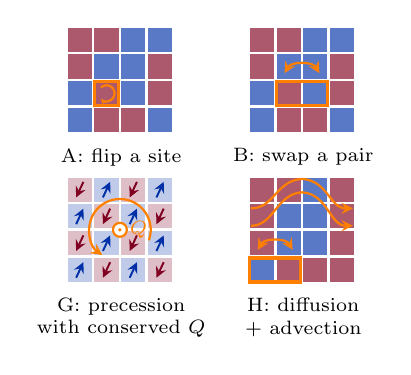
\begin{tikzpicture}[x=0.34cm,y=0.34cm,>=stealth]
        % A, B, H share the scalar +-phi pattern; G is a staggered vector spin pattern
        \foreach \dx/\dy/\lab in {0/0/{A: flip a site},6.8/0/{B: swap a pair}} {
          \begin{scope}[shift={(\dx,\dy)}]
            \foreach \i/\j/\c in {0/0/Kleinblue,1/0/burgundy,2/0/burgundy,3/0/Kleinblue,
                                  0/1/Kleinblue,1/1/burgundy,2/1/Kleinblue,3/1/burgundy,
                                  0/2/burgundy,1/2/Kleinblue,2/2/Kleinblue,3/2/burgundy,
                                  0/3/burgundy,1/3/burgundy,2/3/Kleinblue,3/3/Kleinblue}
              \fill[\c!65] (\i,\j) rectangle ++(0.9,0.9);
            \node[font=\scriptsize,anchor=north] at (2,-0.25) {\lab};
          \end{scope}}
        \draw[very thick,orange] (1,1) rectangle ++(0.9,0.9);
        \draw[-{Stealth[length=2pt,width=2pt]},thick,orange] (1.45,1.45) ++(135:0.3) arc (135:-135:0.3);
        \begin{scope}[shift={(6.8,0)}]
          \draw[very thick,orange] (1,1) rectangle ++(1.9,0.9);
          \draw[<->,thick,orange] (1.3,2.2) to[bend left=60] (2.6,2.2);
        \end{scope}
        \begin{scope}[shift={(0,-5.6)}]
          \foreach \i/\j/\c/\a in {0/0/Kleinblue/65,1/0/burgundy/245,2/0/Kleinblue/65,3/0/burgundy/245,
                                   0/1/burgundy/245,1/1/Kleinblue/65,2/1/burgundy/245,3/1/Kleinblue/65,
                                   0/2/Kleinblue/65,1/2/burgundy/245,2/2/Kleinblue/65,3/2/burgundy/245,
                                   0/3/burgundy/245,1/3/Kleinblue/65,2/3/burgundy/245,3/3/Kleinblue/65} {
            \fill[\c!25] (\i,\j) rectangle ++(0.9,0.9);
            \draw[->,\c,line width=0.7pt] (\i+0.45,\j+0.45) ++(\a+180:0.32) -- ++(\a:0.64);}
          % conserved charge Q (uniform magnetization) points out of the page (odot) and is the rotation axis
          \draw[->,thick,orange] (1.95,1.95) ++(-20:1.15) arc (-20:235:1.15);
          \fill[white] (1.95,1.95) circle (0.26);
          \draw[thick,orange] (1.95,1.95) circle (0.26);
          \fill[orange] (1.95,1.95) circle (0.07);
          \node[font=\scriptsize,orange,anchor=west,inner sep=1pt] at (2.2,1.95) {$Q$};
          \node[font=\scriptsize,anchor=north,align=center] at (2,-0.25) {G: precession\\with conserved $Q$};
        \end{scope}
        % H: a droplet in the matrix; the flow it excites goes around it and carries it
        \begin{scope}[shift={(6.8,-5.6)}]
          \foreach \i/\j/\c in {0/0/Kleinblue,1/0/burgundy,2/0/burgundy,3/0/burgundy,
                                0/1/burgundy,1/1/Kleinblue,2/1/Kleinblue,3/1/burgundy,
                                0/2/burgundy,1/2/Kleinblue,2/2/Kleinblue,3/2/burgundy,
                                0/3/burgundy,1/3/burgundy,2/3/Kleinblue,3/3/burgundy}
            \fill[\c!65] (\i,\j) rectangle ++(0.9,0.9);
          % Kawasaki swap at the interface keeps sum(phi) fixed; the flow passes over the droplet
          \draw[very thick,orange] (0,0) rectangle ++(1.9,0.9);
          \draw[<->,thick,orange] (0.3,1.2) to[bend left=60] (1.6,1.2);
          \draw[->,thick,orange] (0.05,2.1) .. controls (0.9,2.1) and (1.0,3.3) .. (1.95,3.35)
                                 .. controls (2.9,3.3) and (3.0,2.1) .. (3.85,2.1);
          \draw[->,thick,orange] (0.05,2.75) .. controls (0.9,2.75) and (1.0,3.8) .. (1.95,3.85)
                                 .. controls (2.9,3.8) and (3.0,2.75) .. (3.85,2.75);
          \node[font=\scriptsize,anchor=north,align=center] at (2,-0.25) {H: diffusion\\$+$ advection};
        \end{scope}
      \end{tikzpicture}
    \end{column}
    \begin{column}{0.54\textwidth}
      \small\raggedright
      \kb{Same statics, different dynamics}\\[0.2em]
      the equilibrium weight $e^{-S}$ is identical\\[0.1em]
      relaxation time $\tau\sim\xi^{z}$, $\omega(k)\sim k^{z}$\\[0.1em]
      conservation laws and mode couplings determine $z$\\[0.3em]
      \alert{Model B: conserved $\phi$, $z=4-\eta$}\\[0.3em]
      % "A: flip a site" in the cartoon is a single-site Metropolis move, so a local Monte Carlo chain is Model A dynamics
      \alert{a local Monte Carlo update is Model A}\\
      \alert{critical slowing down, $\tau\propto\xi^{z\simeq2}$}
    \end{column}
  \end{columns}
  \refs{%
    \rtag{Classification:} Hohenberg, Halperin, Rev.\ Mod.\ Phys.\ 49, 435 (1977).\quad
    \rtag{Model B exponent:} Halperin, Hohenberg, Ma, PRB 10, 139 (1974).\quad
    \rtag{Model G and chiral QCD:} Rajagopal, Wilczek, Nucl.\ Phys.\ B 399, 395 (1993).\quad
    \rtag{Model H and QCD:} Son, Stephanov, PRD 70, 056001 (2004).}
\end{frame}

% ---------------------------------------------------------------- 3a
% four cells with a parallel layout: the idea, what it delivers, its limit near the critical point
\begin{frame}{How do we compute a field theory when $\xi\to\infty$?}
  \centering\small
  $\displaystyle\langle O\rangle=\frac{1}{Z}\int\mathcal{D}\phi\;O[\phi]\,e^{-S[\phi]}$\par
  \vspace{1em}
  \begin{columns}[T,onlytextwidth]
    \begin{column}{0.48\textwidth}
      \footnotesize\raggedright
      \kb{Markov chain Monte Carlo}\\[0.2em]
      $\phi^{(1)}\to\phi^{(2)}\to\phi^{(3)}\to\cdots$\\
      a chain that leaves $e^{-S}$ invariant\\
      exact up to statistical errors\\
      \alert{$\tau_{\rm int}\propto\xi^{z}$}, critical slowing down
    \end{column}
    \begin{column}{0.48\textwidth}
      \footnotesize\raggedright
      \kb{Tensor renormalization group}\\[0.2em]
      $Z=\mathrm{tTr}\prod_xT_x$\\
      coarse-grain the tensors, $T\to T'$\\
      no sampling, no sign problem
    \end{column}
  \end{columns}
  \vspace{1.4em}
  \begin{columns}[T,onlytextwidth]
    \begin{column}{0.48\textwidth}
      \footnotesize\raggedright
      \kb{Functional renormalization group}\\[0.2em]
      $\partial_k\Gamma_k=\tfrac12\,\mathrm{Tr}\big[\partial_kR_k\,(\Gamma_k^{(2)}+R_k)^{-1}\big]$\\
      from $\Gamma_\Lambda=S$ to $\Gamma_{k\to0}=\Gamma$\\
      exponents, also in real time\\
      \alert{truncation of $\Gamma_k$}
    \end{column}
    \begin{column}{0.48\textwidth}
      \footnotesize\raggedright
      \kb{Generative models}\\[0.2em]
      $\eta\sim\mathcal N(0,1)\ \to\ \phi\sim p_\theta\approx e^{-S}/Z$\\
      trained on samples or on $S$\\
      each sample from fresh noise\\
      \alert{the bias must be measured}
    \end{column}
  \end{columns}
  \refs{%
    \rtag{TRG:} Levin, Nave, PRL 99, 120601 (2007); Kadoh et al., JHEP 05, 184 (2019); Akiyama et al., PRD 104, 034507 (2021); PRD 113, 074502 (2026).\quad
    \rtag{FRG:} Wetterich, PLB 301, 90 (1993); Tan et al., SciPost Phys.\ 12, 026 (2022); Nat.\ Commun.\ 16, 2916 (2025).\quad
    \rtag{Flows:} Albergo, Kanwar, Shanahan, PRD 100, 034515 (2019).\quad
    \rtag{Diffusion models:} Wang, Aarts, Zhou, JHEP 05, 060 (2024); Zhu et al., JHEP 03, 111 (2026).}
\end{frame}

% ================================================================ Part I
\section{Part I: diffusion models and equilibrium sampling}
\subsection{Diffusion model on the lattice}
% ---------------------------------------------------------------- 3b
\begin{frame}{A diffusion model turns noise back into samples}
  \footnotesize\raggedright
  \vspace{-0.4em}
  \kb{Generative model}\quad learn $p(\phi)$ from its samples, then draw new ones

  \vspace{0.4em}
  {\centering
  \begin{tikzpicture}[font=\scriptsize,>=stealth]
    \foreach \t/\i in {0/0,0.01/1,0.03/2,0.08/3,1/4}
      \node[inner sep=0pt] (p\i) at (1.75*\i,0) {\includegraphics[width=1.1cm]{phi4_diffuse_t\t.png}};
    \draw[->,thick,burgundy] ([yshift=0.1cm]p0.north west) -- ([yshift=0.1cm]p4.north east)
      node[midway,above] {forward: add Gaussian noise until nothing of $\phi$ is left};
    \draw[<-,thick,Kleinblue] ([yshift=-0.1cm]p0.south west) -- ([yshift=-0.1cm]p4.south east)
      node[midway,below] {reverse: a Langevin equation with a learned force turns noise back into a sample};
  \end{tikzpicture}\par}
  \vspace{0.3em}
  \small
  % the lower half swaps with the overlay, the figure above never moves
  \begin{onlyenv}<1>
  \kb{Forward}\quad $\phi_t=\phi_0+\Sigma(t)\,\eta$, a heat equation for $p_t$, nothing to learn
  \vspace{-0.3em}
  \begin{equation*}
    \rmd\phi=\sigma^{t}\,\rmd w,\qquad
    \Sigma^2(t)=\frac{\sigma^{2t}-1}{2\ln\sigma},\qquad
    \Sigma(1)\gtrsim\text{data spread}
  \end{equation*}
  \vspace{-0.9em}

  so $p_{t=1}$ is a broad Gaussian, the same whatever $\phi_0$ was
  \end{onlyenv}
  \begin{onlyenv}<2>
  % two displays in one block: squeeze the display skips or the last line hits the footnote
  \setlength{\abovedisplayskip}{3pt}\setlength{\belowdisplayskip}{3pt}%
  \setlength{\abovedisplayshortskip}{0pt}\setlength{\belowdisplayshortskip}{3pt}%
  \kb{Training}\quad approximate the drift by a network
  \begin{equation*}
    s_\theta(\phi_t,t)\approx\nabla_\phi\log p_t(\phi_t)
  \end{equation*}
  it points from the noised $\phi_t$ back to the data $\phi_0$, $-\eta/\Sigma(t)$
  \begin{equation*}
    \mathcal L(\theta)=\Big\langle\big\|\Sigma(t)\,s_\theta(\phi_t,\,t)+\eta\big\|^2\Big\rangle_{t,\phi_0,\eta}
  \end{equation*}
  the network learns by \alert{predicting the noise it was given}
  \end{onlyenv}
  \begin{onlyenv}<3>
  \kb{Reverse}\quad the same diffusion run backwards, with the learned drift
  \vspace{-0.3em}
  \begin{equation*}
    \rmd\phi=-g^2(t)\,s_\theta(\phi,t)\,\rmd t+g(t)\,\rmd\bar w,\qquad
    \frac{\rmd\phi}{\rmd t}=-\tfrac12 g^2(t)\,s_\theta(\phi,t)
  \end{equation*}
  \vspace{-0.9em}

  SDE and ODE share the marginals $p_t$, $g(t)=\sigma^t$
  \end{onlyenv}
  \begin{onlyenv}<4>
  \setlength{\abovedisplayskip}{3pt}\setlength{\belowdisplayskip}{3pt}%
  \setlength{\abovedisplayshortskip}{0pt}\setlength{\belowdisplayshortskip}{3pt}%
  \kb{Irreversible and reversible}\\[0.1em]
  irreversible: each noisy trajectory (SDE)\\
  reversible: probability distribution (ODE)\\[0.4em]
  \kb{Small-time limit}\quad the drift of stochastic quantization: \alert{is it reproduced?}
  \begin{equation*}
    s_\theta(\phi,t\to0)\ \to\ \nabla_\phi\log p_{\rm data}=-\nabla_\phi S[\phi]
  \end{equation*}
  \end{onlyenv}
  \refs{%
    \only<1-3>{%
    \rtag{Reverse-time diffusion:} Anderson, Stoch.\ Proc.\ Appl.\ 12, 313 (1982).\quad
    \rtag{Denoising diffusion:} Ho, Jain, Abbeel, NeurIPS (2020).\quad
    \rtag{Score SDE:} Song et al., ICLR (2021).\quad
    \rtag{DSM:} Vincent, Neural Comput.\ 23, 1661 (2011).}%
    \only<4>{%
    \rtag{Stochastic quantization:} Parisi, Wu, Sci.\ Sin.\ 24, 483 (1981).\quad
    \rtag{DM as stochastic quantization:} Wang, Aarts, Zhou, JHEP 05, 060 (2024); Fukushima, Kamata, JPSJ 94, 031010 (2025); Hirono, Tanaka, Fukushima, arXiv:2403.11262.}}
\end{frame}

% ---------------------------------------------------------------- 3c
% phi4_snapshot_*.png: last configuration (10240th) of 2Dphi4/trainingdata/cfgs_wolff_fahmc_k=*_l=0.022_128^2.jld2,
% 6 px per site, RdBu with red positive, shared colour range +-2.5 as in phi4_diffuse_*.png
% chi_2d_wolff_fahmc_2.pdf: L=16 to 128 version of the 2D susceptibility figure in the kappa_c appendix of arXiv:2607.08505
\begin{frame}{Which theory do we sample?}
  \centering\small
  $\displaystyle S[\phi]=\sum_x\Big[-2\kappa\sum\nolimits_{\mu=1}^{d}\phi_x\phi_{x+\hat\mu}+\phi_x^2+\lambda\big(\phi_x^2-1\big)^2\Big]$\\[0.2em]
  periodic $L^d$ lattice, symmetric under $\phi\to-\phi$\\
  $\lambda\to\infty$ leaves Ising spins $\phi_x=\pm1$, $\lambda=0$ a Gaussian field\par
  \vspace{0.4em}
  \begin{columns}[T,onlytextwidth]
    \begin{column}{0.58\textwidth}
      \centering
      % 6pt gaps: the middle label is wider than its picture and would touch its neighbours
      \begin{tabular}{@{}c@{\hspace{6pt}}c@{\hspace{6pt}}c@{}}
        \includegraphics[width=1.75cm]{phi4_snapshot_k0.26.png} &
        \includegraphics[width=1.75cm]{phi4_snapshot_k0.2705.png} &
        \includegraphics[width=1.75cm]{phi4_snapshot_k0.28.png}\\
        \scriptsize symmetric & \scriptsize critical & \scriptsize broken\\[-0.2em]
        \scriptsize $\kappa=0.26<\kappa_c$ & \scriptsize $\kappa=0.2705\simeq\kappa_c$ & \scriptsize $\kappa=0.28>\kappa_c$
      \end{tabular}\\[0.4em]
      \footnotesize
      \kb{Couplings}\\[0.3em]
      \begin{tabular}{@{}lcc@{}}
        \toprule
        & $\lambda$ & $\kappa_c$\\
        \midrule
        2D & $0.022$ & $0.27088$\\
        3D & $0.9$ & $0.19225$\\
        \bottomrule
      \end{tabular}
    \end{column}
    \begin{column}{0.40\textwidth}
      \centering
      \includegraphics[width=\linewidth]{chi_2d_wolff_fahmc_2}\\[0.1em]
      {\scriptsize 2D, $\lambda=0.022$}
    \end{column}
  \end{columns}
\end{frame}

% ---------------------------------------------------------------- 3d
% mS_joint_3panels.pdf and cumulant_heatmaps_n4_n8.pdf: Figs. 1 and 2 of arXiv:2607.08505
\begin{frame}{Do the samples match HMC in every phase?}
  \vspace{-0.4em}
  \begin{columns}[T,onlytextwidth]
    \begin{column}{0.77\textwidth}
      \includegraphics[width=\linewidth]{mS_joint_3panels}
    \end{column}
    \begin{column}{0.21\textwidth}
      \scriptsize\raggedright
      \kb{2D, $L=128$}\\[0.3em]
      HMC filled\\
      DM dashed
    \end{column}
  \end{columns}
  \vspace{0.9em}
  \begin{columns}[T,onlytextwidth]
    \begin{column}{0.77\textwidth}
      \includegraphics[width=\linewidth]{cumulant_heatmaps_n4_n8}
    \end{column}
    \begin{column}{0.21\textwidth}
      \scriptsize\raggedright
      \kb{Cumulants}\\[0.3em]
      $\kappa_n(x)=\langle\phi_x^n\rangle_c$\\
      at each site $x$\\
      same colour scale
    \end{column}
  \end{columns}
\end{frame}

\subsection{Critical scaling and volume extrapolation}
% ---------------------------------------------------------------- 9
\begin{frame}{Correlation function at the critical point}
  \begin{columns}[T,onlytextwidth]
    \begin{column}{0.46\textwidth}
      \centering
      \includegraphics[width=\linewidth]{prop_k=0.2705_log_log.pdf}\\[0.1em]
      {\scriptsize 2D, $L=128$, $\kappa=0.2705$, $\eta=1/4$}
    \end{column}
    \begin{column}{0.46\textwidth}
      \centering
      \includegraphics[width=\linewidth]{prop_k=0.1923_log_log.pdf}\\[0.1em]
      {\scriptsize 3D, $L=64$, $\kappa=0.1923$, $\eta\simeq0.036$}
    \end{column}
  \end{columns}
  \vspace{0.8em}
  \begin{columns}[T,onlytextwidth]
    \begin{column}{0.31\textwidth}
      \centering
      \kb{Critical scaling}\\[0.3em]
      \footnotesize $G(k)\propto k^{-(2-\eta)}$\\
      $\eta=0$ for a free field
    \end{column}
    \begin{column}{0.31\textwidth}
      \centering
      \kb{2D Ising}\\[0.3em]
      \footnotesize \alert{$\eta=1/4$ resolved}\\
      off the free $1/k^2$
    \end{column}
    \begin{column}{0.31\textwidth}
      \centering
      \kb{3D Ising}\\[0.3em]
      \footnotesize $\eta\simeq0.036$, lines close\\
      DM and HMC coincide
    \end{column}
  \end{columns}
  \vspace{1.0em}
  {\centering\footnotesize the interacting fixed point leaves its fingerprint in $\eta$, and the samples carry it\par}
  \refs{%
    \rtag{Exponents:} Pelissetto, Vicari, Phys.\ Rept.\ 368, 549 (2002); Hasenbusch, J.\ Phys.\ A 32, 4851 (1999).\quad
    Converged models, trained and sampled at the same $L$.}
\end{frame}

% ---------------------------------------------------------------- 13
\begin{frame}{Train on small lattices, sample a lattice never seen}
  \begin{columns}[T,onlytextwidth]
    \begin{column}{0.40\textwidth}
      \centering
      \includegraphics[width=\linewidth]{L64_crossL_3d_k0.1923_multiL_loglog}\\[0.1em]
      {\scriptsize multi-$L$ training $\to L=64$}
    \end{column}
    \begin{column}{0.40\textwidth}
      \centering
      \includegraphics[width=\linewidth]{L64_crossL_3d_k0.1923_singleL_loglog}\\[0.1em]
      {\scriptsize single-$L$ baselines $\to L=64$}
    \end{column}
  \end{columns}
  \vspace{0.6em}
  \begin{columns}[T,onlytextwidth]
    \begin{column}{0.56\textwidth}
      \footnotesize\raggedright
      \kb{3D, $\kappa=0.1923$: $L_{\rm train}\le32\ \Longrightarrow\ L=64$}\\[0.1em]
      $\{4,8,16,32\}$ tracks HMC \alert{down to $k_{\min}$}\\
      $\{4,8\}$ misses the infrared rise\\
      single $L$: $32$ closest, $4$ fails\\
      several volumes teach the infrared
    \end{column}
    \begin{column}{0.42\textwidth}
      \centering
      {\scriptsize
      \renewcommand{\arraystretch}{0.95}
      \setlength{\tabcolsep}{5pt}
      \begin{tabular}{lc}
        \toprule
        training $L$ & acceptance \\
        \midrule
        $\{4,8\}$ & $0.578(8)$ \\
        $\{4,8,16\}$ & $0.830(6)$ \\
        $\{4,8,16,32\}$ & $0.877(6)$ \\
        $\{64\}$, in distribution & $0.911(9)$ \\
        \bottomrule
      \end{tabular}}
    \end{column}
  \end{columns}
  \refs{%
    \rtag{Multi-lattice generative models:} M\'at\'e, Fleuret, MLST 5, 045053 (2024); Bauer, Kapust, Pawlowski, Temmen, SciPost Phys.\ 19, 077 (2025); Singha et al., ICLR (2025); Zhu et al., JHEP 03, 111 (2026).\quad
    \rtag{Cost of large-volume training:} Abbott et al., EPJA 59, 257 (2023).\quad
    No $L=64$ information enters training or sampling.}
\end{frame}

\subsection{QCD sampling}
% ---------------------------------------------------------------- 13b
\begin{frame}{QCD Sampling}
  \begin{columns}[T,onlytextwidth]
    \begin{column}{0.48\textwidth}
      \footnotesize\raggedright
      \kb{4D SU(3)}\quad diffusion on the group\\[0.3em]
      noise multiplies the links $U_\mu(x)$
      \begin{equation*}
        U\to e^{\rmi\,g\sqrt{\Delta t}\,\eta^aT^a}\,U
      \end{equation*}
      Brownian motion on SU(3)\\
      Haar-random links at $t=1$\\[0.3em]
      score $s_\theta^a\approx\nabla^a\log p_t$ in the Lie algebra
      \begin{equation*}
        U\to e^{\rmi\,(g^2s_\theta^a\Delta t+g\sqrt{\Delta t}\,\eta^a)\,T^a}\,U
      \end{equation*}
      reverse steps stay in SU(3)
    \end{column}
    \begin{column}{0.48\textwidth}
      \footnotesize\raggedright
      \kb{Fermions}\quad integrated out
      \begin{equation*}
        p(\phi)\propto\det M[\phi]\;e^{-S[\phi]}
      \end{equation*}
      % Yukawa coupling written y, g is the diffusion coefficient on the left
      \begin{equation*}
        M[\phi]=DD^\dagger,\quad D[\phi]=D_0+y\,\phi
      \end{equation*}
      \begin{equation*}
        s_\theta\xrightarrow{t\to0}-\nabla S+\underbrace{\nabla\log\det M[\phi]}_{\text{nonlocal}}
      \end{equation*}
      learned from HMC samples\\
      generation without $M^{-1}$
    \end{column}
  \end{columns}
  \vspace{1.0em}
  {\footnotesize\raggedright
  \kb{Full QCD}\quad $p(U)\propto\det M[U]\;e^{-S_g[U]}$\\[0.2em]
  links diffuse on SU(3), quarks enter through the training configurations\par}
  \refs{%
    \rtag{Diffusion on manifolds:} De Bortoli et al., NeurIPS (2022).\quad
    \rtag{Diffusion for gauge fields:} Aarts et al., arXiv:2601.19552.\quad
    \rtag{Yukawa model:} Albergo et al., PRD 104, 114507 (2021).}
\end{frame}

% ================================================================ Part II
\section{Part II: real-time critical dynamics}
\subsection{Conserved dynamics on the lattice}
% ---------------------------------------------------------------- 15
\begin{frame}{From statics to dynamics}
  \small
  \begin{columns}[T,onlytextwidth]
    \begin{column}{0.46\textwidth}
      \kb{Statics}\\[0.15em]
      Boltzmann weight $e^{-S[\phi]}$\\[0.15em]
      however it was reached\\[0.15em]
      \alert{no time}
    \end{column}
    \begin{column}{0.52\textwidth}
      \kb{Dynamics}\\[0.15em]
      equation of motion $\partial_t\phi=\mathcal F[\phi,\xi]$\\[0.15em]
      \alert{stochastic trajectories $\phi(t)$}\\[0.15em]
      $\mathcal F$ does not depend on $t$
    \end{column}
  \end{columns}
  % slide 1 only, the hidden overlays below keep their space and are pushed off the page
  \only<1>{%
    \vspace{2.2em}
    {\centering\scriptsize
    \begin{tabular}{@{}c@{\hspace{6pt}}c@{\hspace{6pt}}c@{\hspace{6pt}}c@{}}
      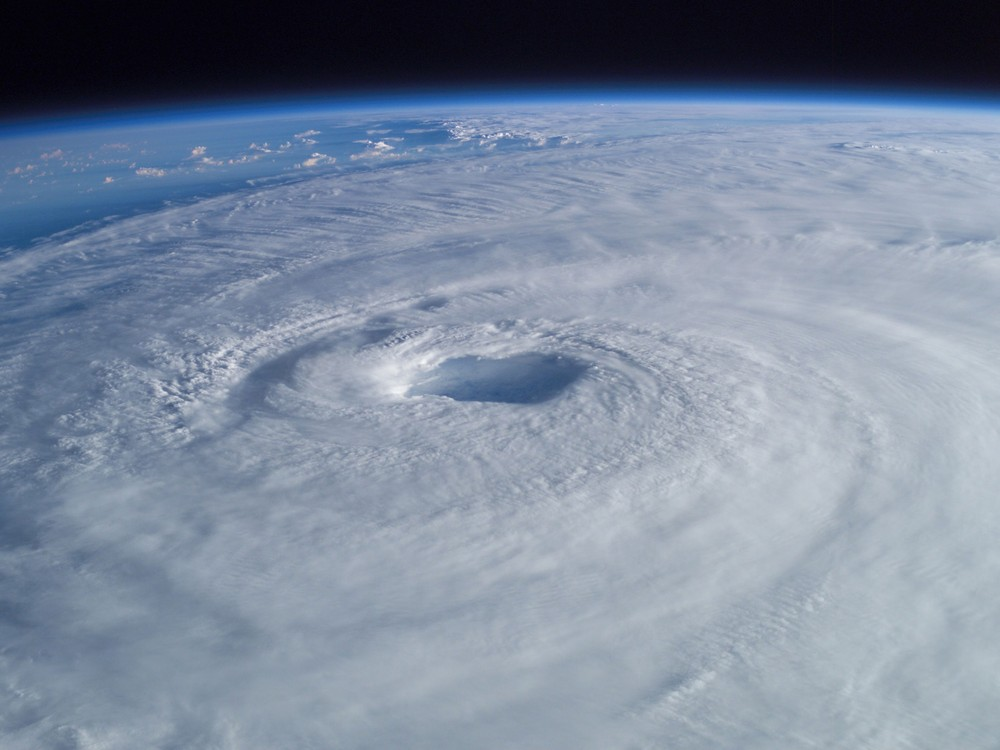
\includegraphics[height=2cm]{hurricane_isabel.jpg} &
      \includegraphics[height=2cm]{myoglobin.png} &
      \includegraphics[height=2cm]{colloid_tracks.png} &
      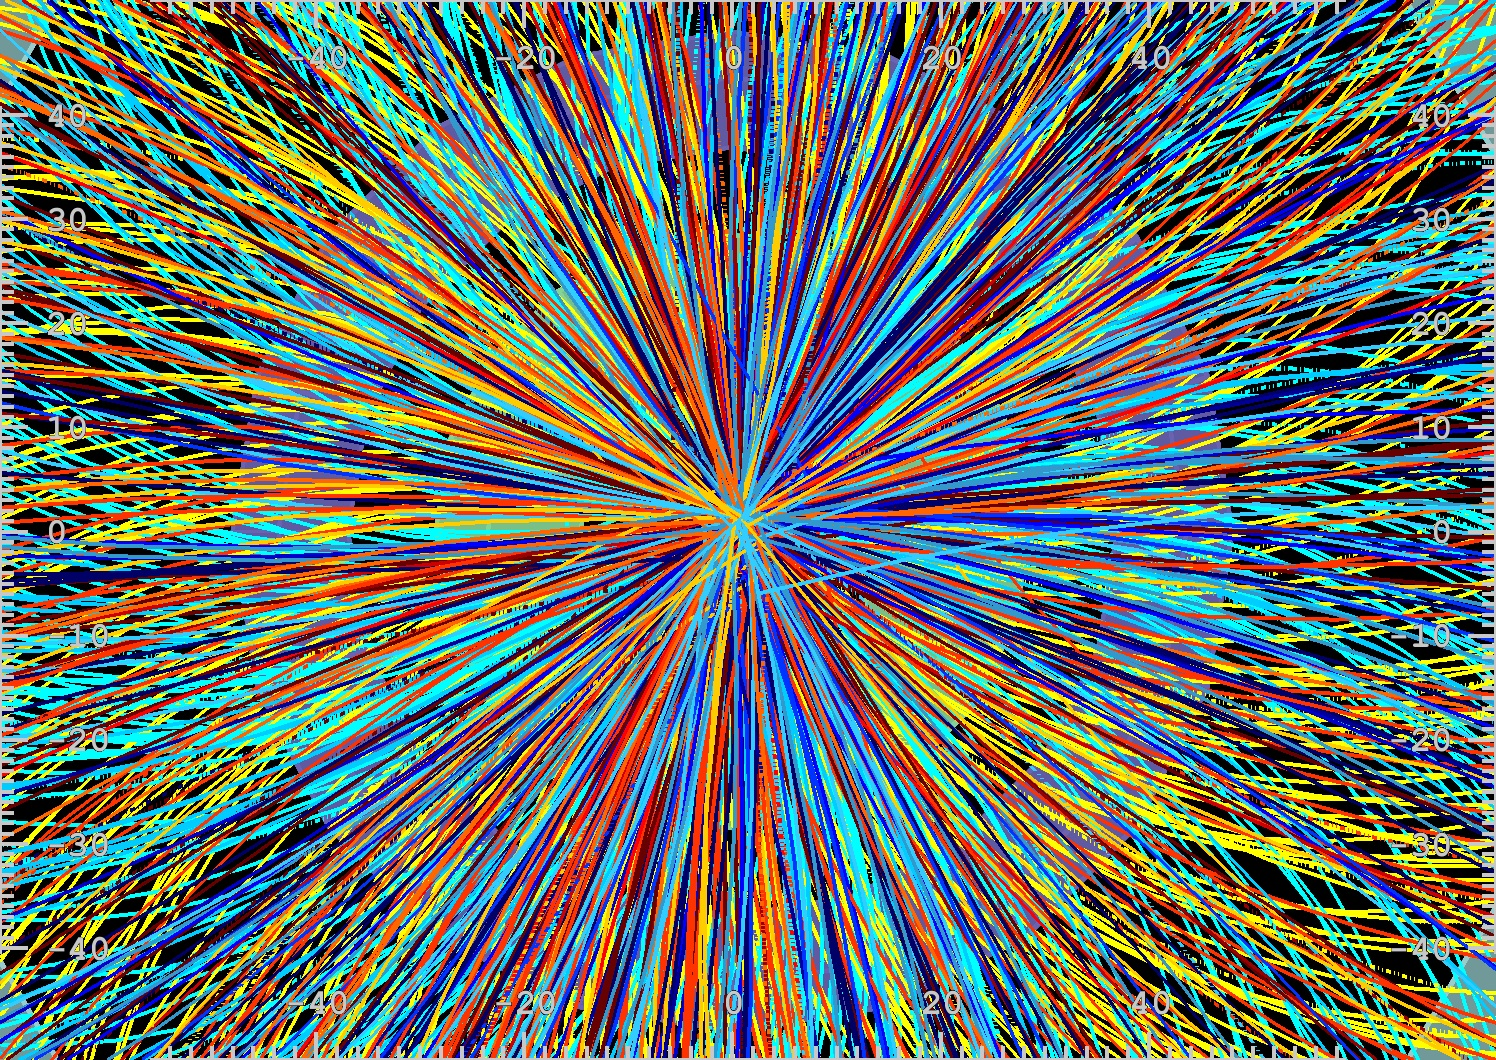
\includegraphics[height=2cm]{alice_pbpb_event.jpg}\\
      weather & protein dynamics & driven colloids & heavy-ion collision
    \end{tabular}\par}
    \refs{%
      \rtag{Hurricane Isabel:} NASA.\quad
      \rtag{Myoglobin:} Wikimedia Commons.\quad
      \rtag{ALICE event display:} CERN.\quad
      \rtag{Colloids:} Dieball et al., Soft Matter 21, 2170 (2025).\quad
      \rtag{Learned kernels:} weather, Price et al., Nature 637, 84 (2025). Proteins, Schreiner, Winther, Olsson, NeurIPS (2023).}}

  \vspace{0.2em}
  \onslide<2->
  \kb{Transition kernel}\quad \alert{$p_{\delta t}(\phi'\,|\,\phi)$}, the probability to go from $\phi$ to $\phi'$ in $\delta t$\par
  \vspace{0.15em}
  \centerline{%
    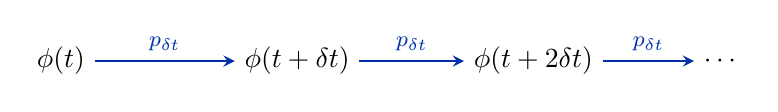
\begin{tikzpicture}[>=stealth]
      \node (a) at (0,0) {$\phi(t)$};
      \node (b) at (3.0,0) {$\phi(t+\delta t)$};
      \node (c) at (6.0,0) {$\phi(t+2\delta t)$};
      \node (d) at (8.4,0) {$\cdots$};
      \foreach \u/\v in {a/b,b/c,c/d}
        \draw[->,thick,Kleinblue] (\u) -- (\v) node[midway,above,font=\footnotesize] {$p_{\delta t}$};
    \end{tikzpicture}}
  \vspace{-0.55em}
  \onslide<3->
  \kb{Learned transition kernel}\\[0.1em]
  \alert{pairs} $(\phi_t,\phi_{t+\delta t})$ suffice, from a simulation or an experiment\\[0.05em]
  \alert{each kernel step spans $\delta t$}, far beyond the step of a direct integrator\\[0.5em]
  \onslide<4->
  \kb{An effective theory in real time}\\[0.1em]
  integrated out: the path between grid times, modes with $\tau_k<\delta t$\\[0.05em]
  $\tau_k\propto k^{-z}$: a longer $\delta t$ is a lower-energy description, $k_{\delta t}\propto\delta t^{-1/z}$
  \refs{%
    \rtag{Chapman--Kolmogorov:} $p_{2\delta t}(\phi'|\phi)=\int\rmd\phi''\,p_{\delta t}(\phi'|\phi'')\,p_{\delta t}(\phi''|\phi)$.\quad
    Colored noise: enlarge the state, $X=(\phi,\eta)$, and the joint kernel composes again.}
\end{frame}

% ---------------------------------------------------------------- 16
\begin{frame}{Model B: conserved dynamics}
  \begin{center}
    2D conserved $\phi^4$ field
  \end{center}
  \begin{columns}[c]
    \begin{column}{0.66\textwidth}
      \begin{align*}
        \partial_t\phi(\bm{x},t)
        &=\Gamma\nabla^2\frac{\delta F[\phi]}{\delta\phi(\bm{x},t)}
          +\zeta(\bm{x},t),\\
        \langle\zeta(\bm{x},t)\zeta(\bm{x}',t')\rangle
        &=-2T\Gamma\nabla^2\delta^{(d)}(\bm{x}-\bm{x}')\delta(t-t'),\\
        F[\phi]
        &=\int d^dx\left[\tfrac{1}{2}(\nabla\phi)^2
        +\tfrac{r}{2}\phi^2+\tfrac{u}{4}\phi^4\right].
      \end{align*}
    \end{column}
    \begin{column}{0.32\textwidth}
      \centering
      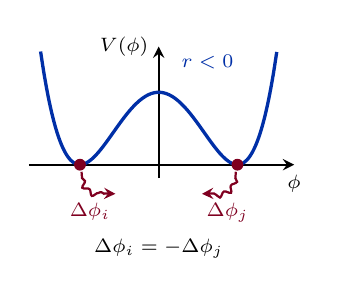
\begin{tikzpicture}[font=\scriptsize,>=stealth]
        % fixes the bounding box below the overlay-2 label, so slide 1 does not jump
        \path (0,-1.1);
        \draw[->,thick] (-1.65,0.25) -- (1.72,0.25) node[below] {$\phi$};
        \draw[->,thick] (0,0.08) -- (0,1.75) node[left] {$V(\phi)$};
        \draw[very thick,Kleinblue,domain=-1.5:1.5,samples=80,smooth]
          plot (\x,{0.25+0.92*(\x*\x-1)^2});
        \node[Kleinblue] at (0.62,1.55) {$r<0$};
        \fill[burgundy] (-1,0.25) circle (0.075);
        \fill[burgundy] (1,0.25) circle (0.075);
        % overlay 2: the conserved exchange; TikZ keeps the bounding box on slide 1
        \draw<2->[->,burgundy,thick,decorate,
              decoration={snake,amplitude=0.3mm,segment length=1.4mm,
                          pre length=0.8mm,post length=1.5mm}]
          (-0.98,0.16) .. controls (-0.98,-0.08) and (-0.84,-0.12) .. (-0.55,-0.12)
          node[midway,below=1pt] {$\Delta\phi_i$};
        \draw<2->[->,burgundy,thick,decorate,
              decoration={snake,amplitude=0.3mm,segment length=1.4mm,
                          pre length=0.8mm,post length=1.5mm}]
          (0.98,0.16) .. controls (0.98,-0.08) and (0.84,-0.12) .. (0.55,-0.12)
          node[midway,below=1pt] {$\Delta\phi_j$};
        \node<2-> at (0,-0.82) {$\Delta\phi_i=-\Delta\phi_j$};
      \end{tikzpicture}
    \end{column}
  \end{columns}
  % align 在 minipage 末尾会丢掉 belowdisplayskip，没有这行下一栏会压到公式
  \vspace{0.6em}
  \begin{uncoverenv}<3->
  \begin{columns}[T,onlytextwidth]
    \begin{column}{0.42\textwidth}
      \centering
      \kb{Conserved mean}\\[0.4em]
      $M(t)\equiv V^{-1}\!\int d^dx\,\phi(\bm{x},t)$\\[0.3em]
      $M(t)=M(0)$
    \end{column}
    \begin{column}{0.30\textwidth}
      \centering
      \kb{Critical dynamics}\\[0.4em]
      $\tau\propto \xi^z\propto k^{-z}$\\[0.3em]
      $z=4-\eta$
    \end{column}
    \begin{column}{0.26\textwidth}
      \centering
      \kb{Kernel interval}\\[0.4em]
      $\delta t=10$\\[0.3em]
      $\gg$ a solver step
    \end{column}
  \end{columns}
  \end{uncoverenv}
  \refs{%
    \rtag{Model B:} Hohenberg, Halperin, Rev.\ Mod.\ Phys.\ 49, 435 (1977).\quad
    Reference trajectories from a direct stochastic integrator (SOSRA) of these equations, on the lattice action of Part I.\quad
    \rtag{Kernel:} $-\Gamma\nabla^2$ in front of $\delta F/\delta\phi$ leaves the equilibrium $e^{-F/T}$ unchanged and sets the dynamics.\quad
    \rtag{Model B for the QCD critical point:} Nahrgang et al., PRD 99, 116015 (2019); Schweitzer, Schlichting, von Smekal, NPB 984, 115944 (2022); Chattopadhyay et al., PRD 108, 074004 (2023).}
\end{frame}

% ---------------------------------------------------------------- 17
\begin{frame}{Conditional diffusion as the transition kernel}
  \begin{columns}[T,onlytextwidth]
    \begin{column}{0.53\textwidth}
      \centering
      \includegraphics[width=\linewidth]{schematic}\\[0.3em]
      {\normalsize $\Delta\phi\sim p_\theta(\,\cdot\mid\phi_t)$
      \qquad
      $\phi_{t+\delta t}=\phi_t+\Delta\phi$}
    \end{column}
    \begin{column}{0.45\textwidth}
      \footnotesize\raggedright
      \kb{Condition}\\[0.1em]
      the present field $\phi_t$

      \vspace{0.25em}
      \kb{Target}\\[0.1em]
      the increment $\Delta\phi$, diffused\\
      and denoised as in Part I

      \vspace{0.25em}
      \kb{Physics learned}\\[0.1em]
      $p(\Delta\phi\,|\,\phi_t)$ from pairs alone\\
      \alert{no drift, noise or free energy}

      \vspace{0.25em}
      \kb{Physics built in}\\[0.1em]
      $\sum_x\Delta\phi_x=0$ by projection\\
      at every step, $M$ conserved exactly
    \end{column}
  \end{columns}
  \vspace{0.2em}
  \begin{uncoverenv}<2->
  {\footnotesize\raggedright
  \kb{Projection, three times}\quad $P\,v=v-\tfrac{1}{V}\sum_x v_x$, no retraining\\[0.3em]
  \makebox[\linewidth]{$\rmd\Delta\phi_s=-g^2(s)\,\alert{P}\,s_\theta(\Delta\phi_s;\phi_t,s)\,\rmd s+g(s)\,\alert{P}\,\rmd\bar w,\qquad
    \Delta\phi_{s=1}=\alert{P}\,\Sigma(1)\,\eta$}\\[0.3em]
  initial noise, score, noise increments: $\sum_x\Delta\phi_x=0$ exactly at every step\par}
  \end{uncoverenv}
  \refs{%
    Same U-Net as in Part I with $\phi_t$ as a second input channel.}
\end{frame}

% ---------------------------------------------------------------- 18
% pair_*.png: one sample of each recipe below, evolved with SOSRA over Δt=10,
% colour scale RdBu ±1.6 (coarsening, L=64, ℓ=8, w=1.5, A=1.3, η=0.2) and ±2.2 (critical, L=32, Z=0.7, m²=0.2, M=0.4)
\newcommand{\pairpanel}[1]{\raisebox{-.5\height}{\includegraphics[width=1.0cm]{#1}}}
\begin{frame}{Training data for the kernel}
  \footnotesize\raggedright
  \vspace{-0.2em}
  \begin{columns}[T,onlytextwidth]
    \begin{column}{0.47\textwidth}
      \footnotesize\raggedright
      \kb{Critical kernel}\quad $\kappa=\kappa_c$, $L=32$\\[0.2em]
      Gaussian field $\chi$ with propagator
      \vspace{-0.4em}
      \begin{equation*}
        \langle\chi_k\,\chi_{-k}\rangle=\frac{1}{Zk^2+m^2},\quad \phi_0=M+\chi
      \end{equation*}
      \vspace{-0.9em}

      $Z$ sets the amplitude, $m^2$ the correlation length, $M$ the mean, all random over a broad range

      \vspace{1.0em}
      \centerline{%
        \begin{tabular}{@{}c@{\hspace{1pt}}c@{\hspace{1pt}}c@{\hspace{1pt}}c@{\hspace{1pt}}c@{}}
          \pairpanel{pair_crit_chi} & $\scriptstyle\rightarrow$ &
          \pairpanel{pair_crit_phi0} & $\scriptstyle\rightarrow$ &
          \pairpanel{pair_crit_phi1}\\[0.1em]
          \scriptsize $\chi$ & & \scriptsize $\phi_0=M+\chi$ & & \scriptsize $\phi_{\delta t}$
        \end{tabular}}
    \end{column}
    \begin{column}{0.51\textwidth}
      \footnotesize\raggedright
      \onslide<2->
      \kb{Coarsening kernel}\quad $\kappa=0.85$, $L\le64$\\[0.2em]
      $g$ Gaussian with $\langle g(\bm{x})\,g(0)\rangle=e^{-\bm{x}^2/2\ell^2}$
      \vspace{-0.4em}
      \begin{equation*}
        \phi_0=A\tanh\!\big(\tfrac{\ell}{w}\,g\big)+\eta\,\xi
      \end{equation*}
      \vspace{-0.9em}

      domains $\pm A$ of size $\ell$, walls of width $w$, white noise $\xi$ of level $\eta$\\
      $\ell$, $w$, $A$, $\eta$ random over a broad range

      \vspace{1.0em}
      \centerline{%
        \begin{tabular}{@{}c@{\hspace{1pt}}c@{\hspace{1pt}}c@{\hspace{1pt}}c@{\hspace{1pt}}c@{\hspace{1pt}}c@{\hspace{1pt}}c@{}}
          \pairpanel{pair_cg_g} & $\scriptstyle\rightarrow$ &
          \pairpanel{pair_cg_tanh} & $\scriptstyle\rightarrow$ &
          \pairpanel{pair_cg_phi0} & $\scriptstyle\rightarrow$ &
          \pairpanel{pair_cg_phi1}\\[0.1em]
          \scriptsize $g$ & & \scriptsize $A\tanh(\tfrac{\ell}{w}g)$ & & \scriptsize $\phi_0$ & & \scriptsize $\phi_{\delta t}$
        \end{tabular}}
    \end{column}
  \end{columns}
  \vspace{0.1em}
  \begin{uncoverenv}<2->
  \kb{Target}\quad Model B (SOSRA) run from $\phi_0$ over $\delta t=10$, $\Delta\phi=\phi_{\delta t}-\phi_0$\\[0.2em]
  \kb{The point}\quad the kernel learns the rule of motion, not trajectories\\
  \alert{every test is an extrapolation}: other ensembles, longer times, larger lattices
  \end{uncoverenv}
  \refs{%
    $Z$ log-uniform in $[0.05,10]$, $m^2\in[0,0.8]$, $M\in[-0.9,0.9]$; $\ell$ log-uniform in $[2,L/3]$, $w\in[0.7,3]$, $A\in[0.8,1.8]$, $\eta\in[0.05,0.35]$, $1/8$ pure noise; $51200$ pairs per $L$.}
\end{frame}

\subsection{Dynamic critical scaling}
% ---------------------------------------------------------------- 19
\begin{frame}{Equilibrium and nonequilibrium evolution}
  \centering
  \includegraphics[width=\textwidth]{validation_L32}\\[0.4em]
  {\small
  $G_n(t)=V^{-1}\big\langle|\phi_n(t)|^2\big\rangle$,\quad
  $\phi_n(t)=\sum_x e^{-\rmi k_n\cdot x}\,\phi(x,t)$,\quad
  $k_n=\tfrac{2\pi n}{L}(1,1)$\\[0.3em]
  $G_1$ for $n=1$, the softest mode,\qquad
  $\Delta M(t)=M(t)-M(0)$\par}
  \vspace{1.2em}
  \begin{columns}[T,onlytextwidth]
    \begin{column}{0.22\textwidth}
      \footnotesize\raggedright
      \kb{Critical point}\\
      2D, $L=32$\\
      strongly coupled
    \end{column}
    \begin{column}{0.29\textwidth}
      \footnotesize\raggedright
      \kb{Initial ensembles}\\
      HMC equilibrium\\
      Gaussian quench
    \end{column}
    \begin{column}{0.26\textwidth}
      \footnotesize\raggedright
      \kb{Composition}\\
      \alert{$\bm{200}$} kernel steps\\
      $t=2000$
    \end{column}
    \begin{column}{0.23\textwidth}
      \footnotesize\raggedright
      \kb{Against SOSRA}\\
      $G_1(t)$ agrees\\
      $M(t)=M(0)$
    \end{column}
  \end{columns}
\end{frame}

% ---------------------------------------------------------------- 20
\begin{frame}{Mode-resolved two-time correlations}
  % 0.50: the rho_n definition is wider than the old 0.46 column
  \begin{columns}[T,onlytextwidth]
    \begin{column}{0.50\textwidth}
      \footnotesize\raggedright
      \kb{Two-time correlation}
      \begin{equation*}
        \rho_n(\Delta t)=
        \frac{V^{-1}\big\langle\operatorname{Re}[\phi_n(t+\Delta t)\,\phi_n^*(t)]\big\rangle_t}
        {\sqrt{\left\langle G_n(t+\Delta t)\right\rangle_t\left\langle G_n(t)\right\rangle_t}}
      \end{equation*}
      $\langle\cdot\rangle_t$ over trajectories and time origins $t$

      \vspace{0.3em}
      \kb{Conserved dynamics is slow}\\[0.1em]
      $\tau_n\propto k_n^{-z}$ with $z\simeq4$:\\
      the softest mode outlives $n=4$\\
      by two orders of magnitude

      \vspace{0.3em}
      \kb{Iterated kernel against SOSRA}\\[0.1em]
      lines: direct integration\\
      markers: kernel, $\delta t=10$ per step\\
      \alert{the same curve for every mode}\\
      then read off $\tau_n$, test $\tau_n\propto k_n^{-z}$
    \end{column}
    \begin{column}{0.48\textwidth}
      \centering
      \includegraphics[width=\linewidth]{rho_L32}\\[0.1em]
      {\scriptsize 2D, $L=32$, critical, diagonal modes $n=1$--$4$}
    \end{column}
  \end{columns}
  \refs{%
    Time origins along the $t=2000$ equilibrium chain of the previous slide. Errors: leave-one-trajectory-out jackknife.}
\end{frame}

% ---------------------------------------------------------------- 21
\begin{frame}{The critical exponent emerges}
  \begin{columns}[T]
    \begin{column}{0.44\textwidth}
      \begin{onlyenv}<1>
      \kb{Relaxation time}
      \small
      \begin{equation*}
        \rho_n(\tau_n)=e^{-1}
      \end{equation*}

      \kb{Dynamic scaling}
      \begin{equation*}
        \rho_n(\Delta t)=f(\Delta t/\tau_n),\qquad
        \tau_n\propto k_n^{-z}
      \end{equation*}
      all modes on a common curve

      \kb{Fits at $L=32$}

      \alert{$\bm{z_{\rm DM}=3.792(19)}$}

      \alert{$\bm{z_{\rm SOSRA}=3.812(20)}$}

      exact: $z=4-\eta=3.75$
      \end{onlyenv}
      \begin{onlyenv}<2>
      \kb{The scaling function}
      \small
      \begin{equation*}
        f(x)=e^{-\lambda_0x}(1+ax)^{-b}
      \end{equation*}
      \footnotesize
      $x=\Delta t/\tau_n$, four modes, one fit\\
      a tail slower than $e^{-x}$

      \small
      \kb{Sum rule}
      \begin{equation*}
        -f'(0^+)=\lambda_0+ab=r
      \end{equation*}
      \footnotesize
      $r=\tau_n\hat k_n^2/G_n$, the initial decay\\
      rate of $\rho_n$, set by the statics\\
      \alert{two free parameters} $\lambda_0$, $a$\\
      $b=(r-\lambda_0)/a$ follows\\
      free fits hit $r$ within a few \%
      \end{onlyenv}
    \end{column}
    \begin{column}{0.54\textwidth}
      \includegraphics[width=0.94\linewidth]{collapse_dm_L32}
      {\fontsize{6}{7}\selectfont
      \textcolor{Kleinblue}{$z=4-\eta=15/4=3.75$}. \rtag{Exact.} Halperin et al., PRB 10, 139 (1974).\\
      \textcolor{Kleinblue}{$z=3.83(10),\ 3.716(17)$}. \rtag{MC.} Schweitzer et al., NPB 984, 115944 (2022).\\
      \textcolor{Kleinblue}{$z=3.95(10)$}. \rtag{Kawasaki MC.} Zheng, PLA 277, 257 (2000), erratum 282, 132 (2001).\\
      \textcolor{Kleinblue}{$z=3.79\pm0.05$}. \rtag{MC RG.} Moseley et al., J. Stat. Phys. 57, 421 (1989).\\
      \textcolor{Kleinblue}{$z=3.80$}. \rtag{MC RG.} Yalabik and Gunton, PRB 25, 534 (1982).
      \par}
    \end{column}
  \end{columns}
\end{frame}

% ---------------------------------------------------------------- 22
\begin{frame}{The scaling function}
  \begin{columns}[T,onlytextwidth]
    \begin{column}{0.44\textwidth}
      \centering
      \includegraphics[width=\linewidth]{gamma_invx_dm_L32}\\[0.1em]
      {\scriptsize decay rate of the learned kernel's $\rho_n$}

      \vspace{0.5em}
      {\footnotesize\raggedright
      \kb{Asymptotics}\\[0.1em]
      \begin{tabular}{@{}l@{\ }l@{}}
        $x\to0$: & $f\simeq1-rx$, $\Gamma_{\rm eff}\to r$\\
        $x\to\infty$: & $f\simeq(ax)^{-b}\,e^{-\lambda_0x}$\\
        & $\Gamma_{\rm eff}\simeq\lambda_0+b/x$, $b\simeq\tfrac12$
      \end{tabular}
      \par}
    \end{column}
    \begin{column}{0.54\textwidth}
      \footnotesize\raggedright
      \kb{The rate runs with the time scale}\\[0.1em]
      $\Gamma_{\rm eff}=-\,d\ln\rho_n/dx$, $x=\Delta t/\tau_n$\\
      free field: eigenmodes, $\Gamma_{\rm eff}=1$\\
      here $\phi_n$ mixes many relaxation modes,\\
      $\Gamma_{\rm eff}$ runs from the bare $r$ to the gap $\lambda_0$

      \vspace{0.25em}
      \kb{Short-time rate from the statics}\\[0.1em]
      fluctuation--dissipation at $\Delta t\to0^+$\\
      $-\rho_n'(0^+)=\Gamma\hat k_n^2T/G_n$, $\Gamma=T=1$\\
      $r=\tau_n\hat k_n^2/G_n\simeq1.8$, $\tau_n$ measured\\
      one $r$ for all modes $\Leftrightarrow\ \tau_n\propto G_n/\hat k_n^2$

      \vspace{0.25em}
      \kb{Long-time rate: a gap}\\[0.1em]
      $\Gamma_{\rm eff}\to\lambda_0\simeq0.27$ from the tail, $x\ge2$\\
      dashed: $\lambda_0+1/(2x)$, $b=\tfrac12$\\
      the sum-rule fit gives $0.33$ instead,\\
      the crossover is approximate
    \end{column}
  \end{columns}
\end{frame}

% ---------------------------------------------------------------- 24
\begin{frame}{Prediction on unseen $L=64$}
  \begin{columns}[T]
    \begin{column}{0.44\textwidth}
      \kb{Size extrapolation}

      \small
      \begin{center}
        $L_{\rm train}=8,16,32$\ \ {$\Longrightarrow$}\ \ \alert{$\bm{L=64}$}\\[0.3em]
        no $L=64$ trajectory ever seen
      \end{center}

      \kb{Fits at $L=64$}

      \alert{$\bm{z_{\rm DM}=3.855(21)}$}

      \alert{$\bm{z_{\rm Model\,B}=3.867(23)}$}

      \vspace{0.6em}
      \kb{As fast as the best direct solver}

      \scriptsize
      512 trajectories, $t=100$, GH200, matched accuracy
    \end{column}
    \begin{column}{0.54\textwidth}
      \centering
      \includegraphics[width=\linewidth,height=0.37\textheight,keepaspectratio]{reverse_nfe_tau_L64}
      \par\vspace{0.3em}
      {\raggedright
        \scriptsize
        \setlength{\tabcolsep}{2pt}
        \begin{tabular}{lcc}
          \toprule
          & \multicolumn{2}{c}{Wall time (s)} \\
          \cmidrule(lr){2-3}
          Method & equil. & noneq. \\
          \midrule
          \alert{DPM-Solver-v3 (This work)} & $3.24$ & $3.26$ \\
          SOSRA (This work) & $1.30$ & $3.28$ \\
          SOSRA (StochasticDiffEq.jl) & $12.36$ & $30.67$ \\
          ShARK (Diffrax) & $5.56$ & $17.76$ \\
          EM (Diffrax) & $19.45$ & $38.75$ \\
          EM (other GPU/CPU solvers) & $>100$ & $>200$ \\
          \bottomrule
        \end{tabular}
      \par}
    \end{column}
  \end{columns}
\end{frame}

\subsection{Phase separation}
% ---------------------------------------------------------------- 25
\begin{frame}{Phase separation on unseen $L=128$}
  \begin{columns}[T]
    \begin{column}{0.44\textwidth}
      \kb{Sign-field correlation}
      \small
      \begin{equation*}
        \sigma(\bm{x},t)=\operatorname{sgn}\phi(\bm{x},t)
      \end{equation*}
      \begin{equation*}
        C(r,t)=\left\langle\sigma(\bm{x},t)\,\sigma(\bm{x}+\bm{r},t)\right\rangle
      \end{equation*}

      $L(t)$: first zero of $C(r,t)$

      \kb{Phase-ordering scaling}
      \begin{equation*}
        C(r,t)=g\big(r/L(t)\big)
      \end{equation*}
      \begin{equation*}
        L(t)\propto t^{1/3}
      \end{equation*}

      \kb{Size extrapolation}

      $L_{\rm train}\le64$\ \ {$\Longrightarrow$}\ \ \alert{$\bm{L=128}$}

      \alert{$\bm{L(t)\propto t^{1/3}}$}\\[0.2em]
      $L_{\rm DM}/L_{\rm SOSRA}=1$ within $2\%$
    \end{column}
    \begin{column}{0.54\textwidth}
      \centering
      \vspace*{-0.6em}
      \includegraphics[width=\linewidth,height=0.50\textheight,keepaspectratio]{collapse_dm_L128}
      \par\vspace{0.15em}
      {\raggedright
      \fontsize{5.2}{5.6}\selectfont
      \textcolor{Kleinblue}{$t^{1/3}$}. \rtag{LSW theory.} Lifshitz and Slyozov, JPCS 19, 35 (1961).\\
      \textcolor{Kleinblue}{Asymptotic $t^{1/3}$, corrections}. \rtag{Conserved Ising.} Huse, PRB 34, 7845 (1986).\\
      \textcolor{Kleinblue}{$t^{1/3}$, scaling}. \rtag{2D critical Model B.} Rogers et al., PRB 37, 9638 (1988).\\
      \textcolor{Kleinblue}{$t^{1/3}$ scaling}. \rtag{Review.} Bray, Adv. Phys. 43, 357 (1994).\\
      \textcolor{Kleinblue}{$t^{1/3}$}. \rtag{Polymer experiment.} Krausch et al., PRL 71, 3669 (1993).\\
      \textcolor{Kleinblue}{Critical $\alpha=1/3$}. \rtag{2D CH.} K\"onig et al., PCCP 23, 24823 (2021).\\
      \textcolor{Kleinblue}{$\alpha_L=0.34,0.37$ from perimeter}. \rtag{Membrane.} Zhiliakov et al., BBA 1863, 183446 (2021).\\
      \textcolor{Kleinblue}{$t^{1/3}$}. \rtag{Passive membrane, CH.} Arnold et al., PRL 131, 128402 (2023).\\
      \textcolor{Kleinblue}{$t^{1/3}$}. \rtag{HP1 Model B.} Tortora et al., PNAS 120, e2211855120 (2023).\\
      \textcolor{Kleinblue}{Long-time $t^{1/3}$}. \rtag{Diffusive polymer Model B.} Garcia et al., JCP 159, 214904 (2023).
      \par}
    \end{column}
  \end{columns}
\end{frame}

\subsection{Colloid experiment}
% ---------------------------------------------------------------- 25b
\begin{frame}{The colloid experiment}
  \begin{columns}[T,onlytextwidth]
    \begin{column}{0.44\textwidth}
      \centering
      % scale 0.8 leaves room for the measured tracks below, text keeps its size
      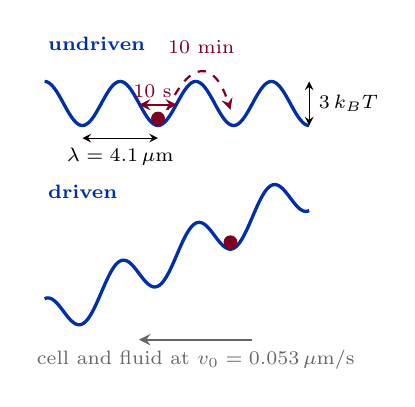
\begin{tikzpicture}[font=\scriptsize,>=stealth,x=1cm,y=1cm,scale=0.8]
        % washboard with period 1.2 cm standing for lambda = 4.1 um, minima at x = 0.6 + 1.2 n
        \node[anchor=west,font=\scriptsize\bfseries\color{Kleinblue}] at (-0.1,0.95) {undriven};
        \draw[very thick,Kleinblue,domain=0:4.2,samples=120,smooth] plot (\x,{0.35*cos(deg(2*pi*\x/1.2))});
        \fill[burgundy] (1.8,-0.24) circle (0.11);
        % xshift keeps the label off the hop arrow at scale 0.8
        \draw[<->,burgundy,thick] (1.5,-0.02) -- (2.1,-0.02) node[midway,above=-1pt,xshift=-2pt] {$10$ s};
        \draw[->,burgundy,thick,dashed] (1.95,-0.1) .. controls (2.3,0.7) and (2.7,0.7) .. (2.95,-0.1)
          node[midway,above=3pt] {$10$ min};
        \draw[<->] (0.6,-0.55) -- (1.8,-0.55) node[midway,below] {$\lambda=4.1\,\mu$m};
        % at the end of the curve, so the label clears it at scale 0.8
        \draw[<->] (4.2,-0.35) -- (4.2,0.35) node[midway,right] {$3\,k_BT$};
        % driven: in the camera frame the fluid moves with the cell, the drag gamma*v0 is a constant force,
        % i.e. a tilted washboard. True tilt is v0*lambda/D = 5.4 kT per period; drawn 0.6 cm = 2.6 kT so the
        % wells stay visible. Arrow lengths: fluid v0 = 1.8 cm, particle v0/2 = 0.9 cm.
        \begin{scope}[yshift=-2.4cm]
          \node[anchor=west,font=\scriptsize\bfseries\color{Kleinblue}] at (-0.1,1.0) {driven};
          \draw[very thick,Kleinblue,domain=0:4.2,samples=160,smooth] plot (\x,{0.35*cos(deg(2*pi*\x/1.2))+0.5*\x-1.05});
          \fill[burgundy] (2.95,{0.35*cos(deg(2*pi*2.95/1.2))+0.5*2.95-1.05+0.11}) circle (0.11);
          \draw[->,thick,black!60] (3.3,-1.35) -- (1.5,-1.35) node[midway,below] {cell and fluid at $v_0=0.053\,\mu$m/s};
        \end{scope}
      \end{tikzpicture}\\
      \includegraphics[height=1.85cm]{colloid_tracks.png}
    \end{column}
    \begin{column}{0.54\textwidth}
      \footnotesize\raggedright
      \kb{The experiment}\\[0.1em]
      polystyrene spheres in a quasi-2D cell\\
      a periodic optical potential along $x$\\
      $1200$ tracks of $30$ to $60$ min

      \vspace{0.3em}
      \kb{Two time scales}\\[0.1em]
      in a well $\sim10$ s, escape $\sim10$ min\\
      the drive tilts the washboard

      \vspace{0.3em}
      \kb{Pairs, as before}\\[0.1em]
      $(r_t,\,r_{t+\delta t})$, $\delta t=10$ s, \alert{first $10$ min only}\\
      condition: the phase in the potential\\
      \alert{no potential, no $D$, no drive is given}

      \vspace{0.3em}
      \kb{Prediction}\\[0.1em]
      iterate from the positions at $10$ min\\
      $300$ steps undriven, $120$ driven
    \end{column}
  \end{columns}
  \refs{%
    \rtag{Experiment:} Dieball et al., Soft Matter 21, 2170 (2025); data: Zenodo 10.5281/zenodo.13908799.\quad
    \rtag{Langevin reference} of the original study: overdamped, $U/k_BT=-\ln p_{\rm eq}$ from the undriven density, $D=0.04\,\mu$m$^2$/s, drift $-v_0$ under driving.}
\end{frame}

% ---------------------------------------------------------------- 25c
\begin{frame}{Transport in the colloid experiment}
  \centering
  \includegraphics[width=0.72\textwidth]{experiment_endmatter}\\[0.1em]
  {\scriptsize top: undriven, bottom: driven. dotted line: end of training}
  \begin{columns}[T,onlytextwidth]
    \begin{column}{0.50\textwidth}
      \footnotesize\raggedright
      \kb{Driven}\quad within $1\%$, Langevin $6\%$ off\\[0.1em]
      \kb{Undriven}\quad drift in (a) is learned,\\
      the equilibrium Langevin has none\\[0.2em]
      \kb{Passage time}\quad first arrival at\\
      $x_{\rm i}\pm\lambda$ undriven, $x_{\rm i}-\lambda$ driven
    \end{column}
    \begin{column}{0.48\textwidth}
      \centering
      {\scriptsize
      \renewcommand{\arraystretch}{0.95}
      \setlength{\tabcolsep}{3pt}
      \begin{tabular}{lcc}
        \toprule
        driven & $\bar v_x$ [$\mu$m/s] & passage [s] \\
        \midrule
        data & $-0.0282(3)$ & $168(4)$ \\
        \alert{learned kernel} & $-0.0284$ & $166.5$ \\
        Langevin & $-0.0298$ & $157.3$ \\
        \bottomrule
      \end{tabular}}
    \end{column}
  \end{columns}
  \refs{%
    (a,e) mean position. (b,f) net displacement over $50$ and $20$ min. (c,g) displacement rate over $10$ s vs phase. (d,h) paths that cross before $t$, $10$ s grid. $32$ replicas per start.}
\end{frame}

\subsection{Outlook}
% ---------------------------------------------------------------- 25d
\begin{frame}{Outlook: stochastic hydrodynamics near the QCD critical point}
  \begin{columns}[T,onlytextwidth]
    \begin{column}{0.36\textwidth}
      \centering
      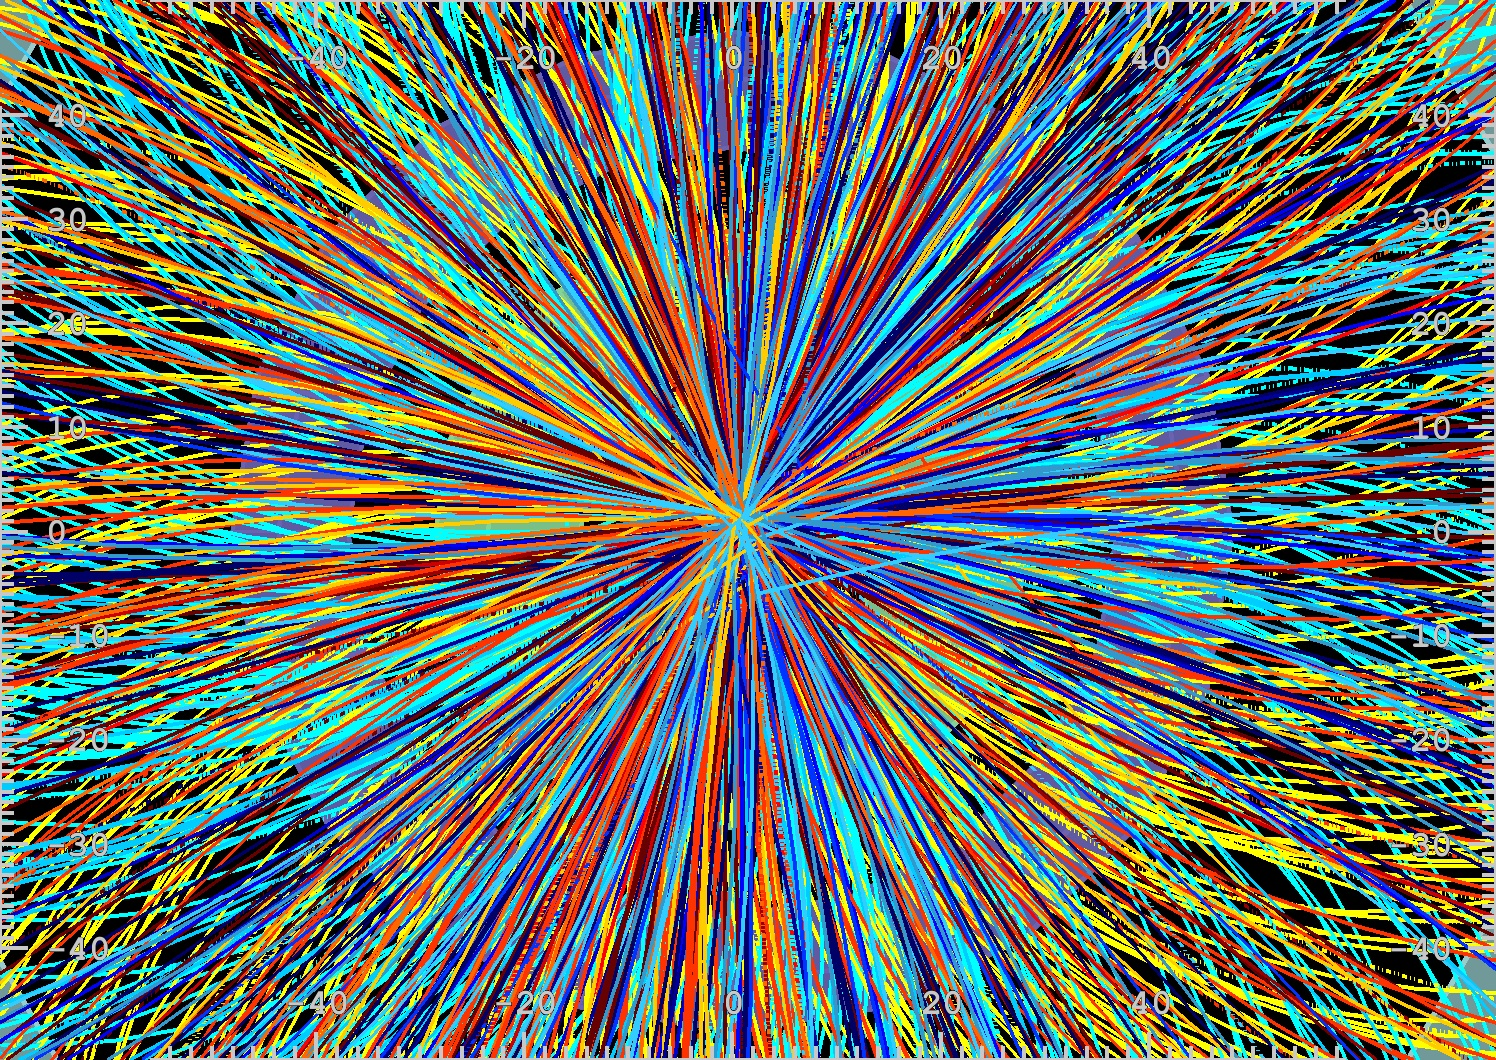
\includegraphics[width=\linewidth]{alice_pbpb_event.jpg}\\[0.1em]
      {\scriptsize ALICE event display, CERN}
    \end{column}
    \begin{column}{0.60\textwidth}
      \footnotesize\raggedright
      \kb{Statics}\quad where is the critical point?\\[0.1em]
      sign problem at $\mu_B\neq0$, lattice, TRG, FRG

      \vspace{0.4em}
      \kb{Beam energy scan}\\[0.1em]
      net-proton cumulants, $\kappa_3\propto\xi^{4.5}$, $\kappa_4\propto\xi^{7}$

      \vspace{0.4em}
      \kb{Dynamics}\quad the fireball never equilibrates\\[0.1em]
      lifetime $\sim10$ fm/$c$, $\tau\sim\xi^{z}$, $\xi$ freezes at $2$--$3$ fm\\
      Model H, $z\simeq3$, $n$ coupled to momentum $\bm\pi$
    \end{column}
  \end{columns}
  \vspace{0.2em}
  \centering
  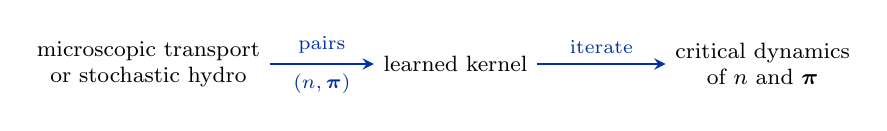
\begin{tikzpicture}[>=stealth, font=\footnotesize, align=center]
    \node (s) at (0,0) {microscopic transport\\ or stochastic hydro};
    \node (k) at (3.9,0) {learned kernel};
    \node (c) at (7.8,0) {critical dynamics\\ of $n$ and $\bm\pi$};
    \draw[->,thick,Kleinblue] (s) -- (k) node[midway,above,font=\scriptsize] {pairs} node[midway,below,font=\scriptsize] {$(n,\bm\pi)$};
    \draw[->,thick,Kleinblue] (k) -- (c) node[midway,above,font=\scriptsize] {iterate};
  \end{tikzpicture}\\[0.3em]
  % the no-modelling claim holds only for microscopic pairs, a hydro source has noise and Gamma put in by hand
  {\footnotesize
  \begin{tabular}{@{}r@{\quad}l@{}}
    \kb{from transport} & \alert{no noise, $\Gamma$ or mode couplings to model}\\
    \kb{from stochastic hydro} & long steps, lattices beyond the training size
  \end{tabular}\par}
  \refs{%
    \rtag{Critical endpoint:} QCD with FRG, Fu, Pawlowski, Rennecke, PRD 101, 054032 (2020); $\mathbb{Z}_3$ gauge-Higgs with TRG, Akiyama, Kuramashi, JHEP 10, 077 (2023).\quad
    \rtag{Non-Gaussian cumulants:} Stephanov, PRL 102, 032301 (2009).\quad
    \rtag{Beam energy scan:} STAR, PRL 126, 092301 (2021).\quad
    \rtag{Critical slowing down:} Berdnikov, Rajagopal, PRD 61, 105017 (2000); Tan et al., PRD 114, L011501 (2026).\quad
    \rtag{Model H:} Son, Stephanov, PRD 70, 056001 (2004).}
\end{frame}

% ---------------------------------------------------------------- 26
\begin{frame}{Summary}
  \centering\small
  \vspace{-0.4em}
  % every picture row is 2.0cm tall, a strut pads the smaller top-left pair, so the text under them lines up across columns
  \begin{columns}[T,onlytextwidth]
    \begin{column}{0.48\textwidth}
      \centering
      \rule{0pt}{2.0cm}%
      \begin{tikzpicture}[>=stealth]
        \node[inner sep=0pt] (a) at (0,0) {\includegraphics[height=1.3cm]{phi4_diffuse_t1.png}};
        \node[inner sep=0pt] (b) at (2.2,0) {\includegraphics[height=1.3cm]{phi4_diffuse_t0.png}};
        \draw[<->,thick,Kleinblue] (a) -- (b);
      \end{tikzpicture}\\
      \kb{A diffusion model learns the\\ drift of stochastic quantization}
    \end{column}
    \begin{column}{0.48\textwidth}
      \centering
      \includegraphics[height=2.0cm]{schematic}\\
      \kb{A conditional diffusion model\\ learns the transition kernel}
    \end{column}
  \end{columns}
  \vspace{1.3em}
  \begin{columns}[T,onlytextwidth]
    \begin{column}{0.48\textwidth}
      \centering
      \includegraphics[height=2.0cm]{collapse_dm_L32}\\
      \kb{Long-time universality emerges\\ from short-time pairs}\\[0.2em]
      $\delta t\ll\tau\sim\xi^{z}$
    \end{column}
    \begin{column}{0.48\textwidth}
      \centering
      \includegraphics[height=2.0cm]{qcd_phase_diagram_bhalerao.png}\\
      \kb{Next, stochastic hydrodynamics\\ near the QCD critical point}\\[0.2em]
      from microscopic $(n,\bm\pi)$ pairs
    \end{column}
  \end{columns}
  % pinned in the band \refs uses on other slides, so the four pictures get the full height
  \begin{tikzpicture}[remember picture, overlay]
    \node[anchor=south, font=\large] at ([yshift=0.45cm]current page.south) {Thank you!};
  \end{tikzpicture}
\end{frame}

\appendix
\section{Backup}
% ---------------------------------------------------------------- 6
\begin{frame}{Score network and reference configurations}
  \centering
  \only<1>{\includegraphics[width=0.92\textwidth]{architecture_ncsnpp_v2}}%
  \only<2->{\includegraphics[width=0.6\textwidth]{architecture_ncsnpp_v2}}
  \vspace{0.1em}
  % left column: the physics (put in by hand vs learned); right column: how it is realised
  \begin{columns}[T,onlytextwidth]
    \begin{column}{0.48\textwidth}
      \footnotesize\raggedright
      \kb{Physics built in}\\[0.1em]
      periodic lattice: circular padding\\
      translation symmetry: convolutions\\
      \alert{nothing else}, not even $\phi\to-\phi$
    \end{column}
    \begin{column}{0.50\textwidth}
      \footnotesize\raggedright
      \kb{Architecture}\\[0.1em]
      U-Net, $L\to L/8$: reaches the infrared\\
      skip connections keep the ultraviolet\\
      no dense layer: any $L$, same weights
    \end{column}
  \end{columns}
  % [T] columns pull their content up by 1ex, so the skip must be larger than it looks
  \vspace{0.7em}
  \begin{uncoverenv}<2->
  \begin{columns}[T,onlytextwidth]
    \begin{column}{0.48\textwidth}
      \footnotesize\raggedright
      \kb{Physics learned}\\[0.1em]
      the action $S[\phi]$, never given\\
      the $\phi\to-\phi$ symmetry\\
      critical correlations, which phase
    \end{column}
    \begin{column}{0.50\textwidth}
      \footnotesize\raggedright
      \kb{Reference configurations}\\[0.1em]
      HMC with Wolff reflections\\
      $\kappa$ below, at and above $\kappa_c$\\
      $10240$ / $2560$ configs, \alert{all it ever sees}
    \end{column}
  \end{columns}
  \end{uncoverenv}
  \refs{%
    \rtag{NCSN++:} Song et al., ICLR (2021).\quad
    The noise level $t$ enters every Res Block through an embedding, panel (b).\quad
    $\kappa_c=0.27088$ (2D, $L=128$), $0.19225$ (3D, $L=64$) from Binder crossings; 3D: Hasenbusch, J.\ Phys.\ A 32, 4851 (1999).}
\end{frame}

\end{document}
